\documentclass{article}
\usepackage[margin=1in]{geometry}
\usepackage{amsmath}
\usepackage{amssymb}
\usepackage{amsthm}
\usepackage{graphicx}
\usepackage{booktabs}
\usepackage{hyperref}
\usepackage{float}
\usepackage{caption}
\usepackage{subcaption}
\usepackage{tikz}
\usetikzlibrary{positioning}
%\usepackage{newtxtext,newtxmath} % Times-like font
\usepackage{mathpazo} % Palatino font
%\usepackage{libertinus} % Libertinus font
\usepackage{pgfplots}
\pgfplotsset{compat=1.17} % or 1.18, etc.
\usepackage{pgf-pie} % pie charts
\usepgfplotslibrary{statistics}
\usepackage{enumitem}
\usepackage{tcolorbox}
\tcbuselibrary{breakable}
\usepackage{fancyhdr}
\pagestyle{fancy}
\fancyhf{}

\theoremstyle{definition}
\newtheorem{definition}{Definition}[section]
\newtheorem{example}{Example}[section]
\newtheorem{properties}{Properties}[section]
\theoremstyle{plain}
\newtheorem{theorem}{Theorem}[section]

\newenvironment{flushlefttab}{
  \begin{flushleft}
  \begin{tabular}{@{} l p{0.75\textwidth} @{}}}
  {\end{tabular}
  \end{flushleft}}



\setlength{\parindent}{0pt}





\definecolor{light-gray}{gray}{0.95}
\definecolor{light-blue}{RGB}{210,225,255}
\definecolor{light-yellow}{RGB}{255, 255, 210}

\newenvironment{ideaBox}{\begin{center}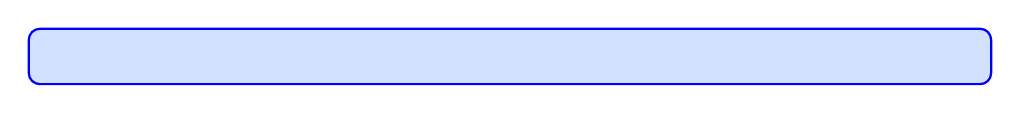
\begin{tikzpicture}
\node[fill=light-blue, draw=blue, thick, rounded corners, inner sep=10pt, text width=0.95\textwidth] \bgroup\footnotesize}{\egroup;\end{tikzpicture}\end{center}}

\newenvironment{warningBox}{\begin{center}
\begin{tikzpicture}
\node[fill=light-yellow, draw=orange, thick, rounded corners, inner sep=10pt, text width=0.95\textwidth] \bgroup\footnotesize}{\egroup;\end{tikzpicture}\end{center}}


\pagestyle{fancy}
\fancyhf{}
\rhead{AP Statistics Unit 2}
\lhead{Exploring Two-Variable Data}
\cfoot{\thepage}

\title{\vspace{-2cm}AP Statistics -- Unit 2\\Exploring Two-Variable Data}
\date{}


\begin{document}

\maketitle

\section*{2.1 Introducing Statistics: Relationships Between Variables}
Often, data will involve several variables that may be related to one another. Here we want to begin discussing relationships between two variables. 

\begin{tcolorbox}[title=Key Terms, colback=blue!5!white, colframe=blue!75!black, breakable]
When dealing with two-variable data, we denote an \textbf{explanatory variable} $x$ and a \textbf{response variable} $y$.
\end{tcolorbox}
\par\medskip

\begin{tcolorbox}[title=Key Terms, colback=blue!5!white, colframe=blue!75!black, breakable]
Two variables may be related in the following ways:
\begin{itemize}
    \item \textbf{Positive association}: As $x$ increases, $y$ increases too.
    \item \textbf{Negative association}: As $x$ increases, $y$ decreases.
    \item \textbf{No association}: Changes in $x$ do not systematically affect $y$.
\end{itemize}
\end{tcolorbox}

\begin{figure}[H]
    \centering
    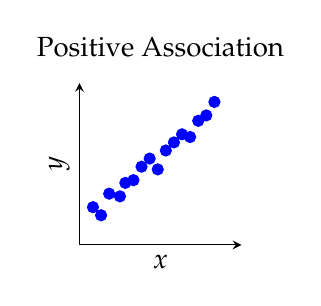
\begin{tikzpicture}
        \begin{axis}[
            width=0.3\textwidth,
            height=0.3\textwidth,
            title={Positive Association},
            xlabel={$x$},
            ylabel={$y$},
            xmin=0, xmax=6,
            ymin=0, ymax=6,
            axis lines=left,
            ticks=none,
            xtick=\empty,
            ytick=\empty
        ]
        \addplot[only marks, mark=*, blue]
        coordinates {
            (0.5,1.4) (0.8,1.1) (1.1,1.9) (1.5,1.8) (1.7,2.3) (2.0,2.4) (2.3,2.9) (2.6,3.2)
            (2.9,2.8) (3.2,3.5) (3.5,3.8) (3.8,4.1) (4.1,4.0) (4.4,4.6) (4.7,4.8) (5.0,5.3)
        };
        \end{axis}
    \end{tikzpicture}
    \hspace{0.5cm}
    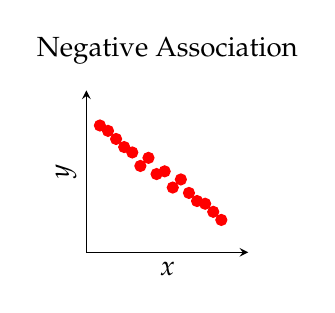
\begin{tikzpicture}
        \begin{axis}[
            width=0.3\textwidth,
            height=0.3\textwidth,
            title={Negative Association},
            xlabel={$x$},
            ylabel={$y$},
            xmin=0, xmax=6,
            ymin=0, ymax=6,
            axis lines=left,
            ticks=none,
            xtick=\empty,
            ytick=\empty
        ]
        \addplot[only marks, mark=*, red]
        coordinates {
            (0.5,4.7) (0.8,4.5) (1.1,4.2) (1.4,3.9) (1.7,3.7) (2.0,3.2) (2.3,3.5) (2.6,2.9)
            (2.9,3.0) (3.2,2.4) (3.5,2.7) (3.8,2.2) (4.1,1.9) (4.4,1.8) (4.7,1.5) (5.0,1.2)
        };
        \end{axis}
    \end{tikzpicture}
    \hspace{0.5cm}
    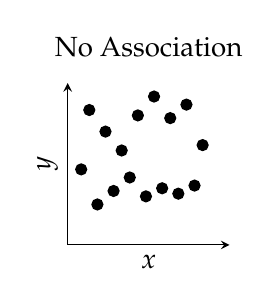
\begin{tikzpicture}
        \begin{axis}[
            width=0.3\textwidth,
            height=0.3\textwidth,
            title={No Association},
            xlabel={$x$},
            ylabel={$y$},
            xmin=0, xmax=6,
            ymin=0, ymax=6,
            axis lines=left,
            ticks=none,
            xtick=\empty,
            ytick=\empty
        ]
        \addplot[only marks, mark=*, black]
        coordinates {
            (0.5,2.8) (0.8,5.0) (1.1,1.5) (1.4,4.2) (1.7,2.0) (2.0,3.5) (2.3,2.5) (2.6,4.8)
            (2.9,1.8) (3.2,5.5) (3.5,2.1) (3.8,4.7) (4.1,1.9) (4.4,5.2) (4.7,2.2) (5.0,3.7)
        };
        \end{axis}
    \end{tikzpicture}
    \caption*{Types of Association Between Two Variables}
\end{figure}



\section*{2.2 Constructing and Interpreting Scatterplots}

\textbf{Scatterplots} display two quantitative variables measured on the same individuals.

\textbf{To describe a scatterplot:}
\begin{itemize}
    \item \textbf{Direction}: Positive, negative, or no association
    \item \textbf{Form}: Linear, curved, clusters, etc.
    \item \textbf{Strength}: Strong, moderate, or weak association
    \item \textbf{Outliers}: Points that fall outside the general pattern
\end{itemize}
Interpretation: ``There is a strong/moderate/weak positive/negative linear relationship between (explanatory variable) and (response variable)."

\begin{example}
\textbf{Example:} Describe the association shown in a scatterplot of study hours (\(x\)) vs. exam scores (\(y\)).

\textit{Solution:} Positive, linear, moderately strong association with one outlier.
\end{example}

\section*{2.3 Correlation}

The \textbf{correlation coefficient} \(r\) measures the strength and direction of a linear relationship between two quantitative variables.

\begin{itemize}
    \item \(r\) is between \(-1\) and \(1\)
    \item \(r>0\): Positive association, \quad \(r<0\): Negative association
    \item The closer \(r\) is to \(\pm1\), the stronger the linear relationship
\end{itemize}

\begin{warningBox}
\textbf{Important:} Correlation \textbf{does not imply causation}.
\end{warningBox}
Interpretation: ``The correlation $r$ shows/confirms that there is a strong/moderate/weak linear relationship between (explanatory variable) and (response variable)."

\begin{example}
\textbf{Example:} A correlation of \(r=0.85\) suggests a strong positive linear relationship.
\end{example}

\section*{2.4 Least Squares Regression Lines (LSRL)}

The \textbf{LSRL} predicts values of the response variable \(y\) given an explanatory variable \(x\).

Equation: \[ \hat{y} = a + bx \]
where:
\begin{itemize}
    \item \(b = r \times \dfrac{s_y}{s_x}\) (slope)
    \item \(a = \bar{y} - b\bar{x}\) (y-intercept)
\end{itemize}

\begin{ideaBox}
\textbf{Interpretation of Slope:} For each additional unit increase in \(x\), the predicted \(y\) increases/decreases by \(b\) units.

\textbf{Interpretation of Intercept:} The predicted \(y\) when \(x=0\).
\end{ideaBox}

\section*{2.5 Residuals}

A \textbf{residual} is the difference between an observed \(y\) and the predicted \(\hat{y}\):
\[ \text{Residual} = y - \hat{y} \]

\begin{itemize}
    \item Positive residual: Actual \(y\) is above the predicted \(\hat{y}\)
    \item Negative residual: Actual \(y\) is below the predicted \(\hat{y}\)
\end{itemize}

Residual plots help assess whether a linear model is appropriate.

\section*{2.6 Assessing the Fit: $r^2$ and Standard Deviation of Residuals}

\textbf{Coefficient of Determination} (\(r^2\)) tells the percent of the variation in \(y\) explained by the model.

\textbf{Standard Deviation of Residuals} (\(s\)) measures the typical distance between the observed \(y\)-values and the predicted \(\hat{y}\)-values.

\begin{example}
\textbf{Example:} If \(r^2 = 0.72\), then 72\% of the variation in \(y\) is explained by the linear model relating \(x\) to \(y\).
\end{example}

\section*{Practice Problems}

\begin{enumerate}
    \item Suppose the correlation between hours of exercise and weight loss is \(r = -0.64\).
    \begin{itemize}
        \item (a) Describe the direction and strength.
        \item (b) Is weight loss caused by exercise based on this information alone?
    \end{itemize}

    \vspace{0.5em}
    \textit{Solution:}
    \begin{itemize}
        \item (a) The relationship is moderately strong and negative.
        \item (b) No, correlation does not imply causation.
    \end{itemize}

    \item A least squares regression line for predicting exam score (\(y\)) from study hours (\(x\)) is \(\hat{y} = 50 + 5x\).
    \begin{itemize}
        \item (a) Interpret the slope.
        \item (b) Predict the score for someone who studies 6 hours.
    \end{itemize}

    \vspace{0.5em}
    \textit{Solution:}
    \begin{itemize}
        \item (a) Each additional hour of study is associated with a predicted increase of 5 points.
        \item (b) \(\hat{y} = 50 + 5(6) = 80\).
    \end{itemize}

    \item Given the residual plot below shows a clear curved pattern, what conclusion can you draw?

    \vspace{0.5em}
    \textit{Solution:} The relationship between \(x\) and \(y\) is not linear; a different model may be more appropriate.
\end{enumerate}

\end{document}
